\documentclass[letterpaper]{article}
\usepackage[T1]{fontenc}
\usepackage[utf8]{inputenc}
\usepackage{tocloft,siunitx,amssymb,amsmath,graphicx,subcaption,float}
\usepackage[top=3cm,left=3cm,right=3cm]{geometry}
\usepackage[american]{circuitikz}
\graphicspath{{img/}}
\renewcommand\cftsecfont{\normalfont}
\renewcommand\cftsecpagefont{\normalfont}
\renewcommand{\cftsecleader}{\cftdotfill{\cftsecdotsep}}
\renewcommand\cftsecdotsep{\cftdot}
\renewcommand\cftsubsecdotsep{\cftdot}
\renewcommand\cftsubsubsecdotsep{\cftdot}
\title{Lab 7: Voltage Divider}
\author{
    Sebastián Nava López\\
    \and
    Ericka Sabrina Pensamiento R.\\
    \and
    Salvador Palos Gil
}
%\captionsetup[subfigure]{justification=raggedright}
\begin{document}
\begin{titlepage}
    \centering
    {\Huge Instituto Politécnico Nacional}\\[3ex]
    {\huge Escuela Superior de Cómputo}\\[8ex]
    {\huge Fundamental Circuit Analysis}\\[12ex]
    {\Large Lab 7: Voltage Divider(DC)}\\[20ex]
    {\Large Group: 1CV5 Team: 7 \\[8ex]
    Sebastian Nava López\\[4ex]
    Sabrina Erika Pensamiento Robledo\\[4ex]
    Salvador Palos Gil\\[18ex]
    }
    \large{Elaboration: May 8, 2018 \hspace{8em} Due date: May 18, 2018}
\end{titlepage}
\tableofcontents
\newpage
\section{Introduction}
In electronics, a voltage divider (also known as a potential divider) is a passive linear circuit that
produces an output voltage ($V_{out}$) that is a fraction of its input voltage ($V_{in}$). Voltage division is the
result of distributing the input voltage among the components of the divider. A simple example of a
voltage divider is two resistors connected in series, with the input voltage applied across the resistor
pair and the output voltage emerging from the connection between them.
\begin{figure}[H]
    \centering
    \begin{circuitikz}
        \draw (2,0) node[ground]{}
        to [R = $Z_1$,-*] (2,2)
        to [R = $Z_2$] (2,4) 
        to [short,-o](0,4)
        (2,2) to [short,-o] (3,2)
        ;
        \draw{
            (3,2) [anchor = south west] node {$V_{out}$}
            (0,4) [anchor = south east] node {$V_{in}$}
        };
    \end{circuitikz}
    \caption{Voltage divider}
    \label{fig:intr1}
\end{figure}
Resistor voltage dividers are commonly used to create reference voltages, or to reduce the
magnitude of a voltage so it can be measured, and may also be used as signal attenuators at
low frequencies. For direct current and relatively low frequencies, a voltage divider may be
sufficiently accurate if made only of resistors; where frequency response over a wide range is
required (such as in an oscilloscope probe), a voltage divider may have capacitive elements
added to compensate load capacitance. In electric power transmission, a capacitive voltage
divider is used for measurement of high voltage.
A voltage divider referenced to ground is created by connecting two electrical impedances in
series, as shown in figure \ref{fig:intr1}. The input voltage is applied across the series
impedances $Z_1$ and $Z_2$ and the output is the voltage across $Z_2$. $Z_1$ and $Z_2$ may 
be composed of any combination of elements such as resistors, inductors and capacitors.
If the current in the output wire is zero then the relationship between the input voltage, $V_{in}$, and
the output voltage, $V_{out}$, is:
\begin{equation}
    V_{out} = \frac{Z_2}{Z_1+Z_1}\cdot V_{in}
    \tag{Voltage divider equation}
\end{equation}
\subsection*{Proof using Ohm's Law}
If $V_{in}$ is given by:
\[V_{in} = I\cdot(Z_1+Z_2)\]
then:
\[I = \frac{V_{in}}{Z_1+Z_2}\]
also, $V_{out}$ is given by:
\[V_{out} = I\cdot Z_2\]
finally:
\[\therefore V_{out} =V_{in}\cdot\frac{Z_2}{Z_1+Z_1}\]
The transfer function (also known as the divider's voltage ratio) of this circuit is:
\[H = \frac{V_{out}}{V_{in}} = \frac{Z_2}{Z_1+Z_1}\]
\section{Development}
\subsection{Voltage divider}
\subsubsection{Calculations}
The circuit is represented in the diagram in figure \ref{fig:diag1}
\begin{figure}[H]
    \centering
    \begin{circuitikz}[scale=0.75,transform shape]
        \draw (0,1) node[ground]{}
        to [V = $V_s:\SI{10}{\volt}$,invert] (0,7.5) to [short,-*] (2,7.5)
        to [R = $R_1:\SI{1}{\kilo\ohm}$,-*](2,5)
        to [R = $R_2:\SI{470}{\ohm}$,-*](2,2.5)
        to [R = $R_3:\SI{560}{\ohm}$](2,1)
        to (2,1) node[ground]{}
        (2,2.5) -- (4.5,2.5) 
        to [R=$R_4:\SI{1}{\kilo\ohm}$](4.5,1)
        to (4.5,1) node[ground]{};
        \draw{ 
            (2,7.5) [anchor = north west] node {$V_1$}
            (2,5) [anchor = north west] node {$V_2$}
            (2,2.5) [anchor = south west] node {$V_3$}
        };
    \end{circuitikz}
    \caption{Circuit diagram}
    \label{fig:diag1}
\end{figure}
As our circuit is composed by resistor wired mostly in series, we can use the voltage 
divider equation to calculate the current between nodes. The voltage divider equation is:
\begin{equation}
    V_{Rx} = R_x\cdot\frac{V_T}{R_{eqT}}
    \label{eq:voltagediv}
\end{equation}
where $R_x$ is the resistor in which we want to measure voltage, $V_T$ is the total voltage in the
circuit, $R_{eqT}$ is the total equivalent resistor in the ciruit.
In this circuit, $V_T$ is equal to $\SI{10}{\volt}$, $R_{eqT}$ is given by:
\begin{align*}
    R_{eqT} &= R_1+R_2+\frac{1}{R_3+R_4}\\
    &=
    \SI{1}{\kilo\ohm}+\SI{470}{\ohm}+\frac{1}{\frac{1}{\SI{560}{\ohm}}+\frac{1}{\SI{1}{\kilo\ohm}}}\\
    &=\SI{1470}{\ohm}+\SI{358.974}{\ohm}\\
    \therefore R_{eqT} &= \SI{1828.974}{\ohm}
\end{align*}
Now we can calculate voltage in each resistor, using \eqref{eq:voltagediv} in $R_1$:
\[V_{R1} = R_1\cdot\frac{V_T}{ReqT} =
\SI{1}{\kilo\ohm}\cdot\frac{\SI{10}{\volt}}{\SI{1828.974}{\ohm}}\qquad\therefore V_{R1} = \SI{5.467}{\volt}\]
In $R_2$:
\[V_{R2} = R_2\cdot\frac{V_T}{ReqT} =
\SI{470}{\ohm}\cdot\frac{\SI{10}{\volt}}{\SI{1828.974}{\ohm}}\qquad\therefore V_{R2} = \SI{2.570}{\volt}\]
As $R_3$ and $R_4$ are connected in parallel, its voltage is the same and is calculated using the
combined resistance of both resistors:
\[V_{R3} = \frac{1}{R_3+R_4}\cdot\frac{V_T}{ReqT} =
\SI{358.974}{\ohm}\cdot\frac{\SI{10}{\volt}}{\SI{1828.974}{\ohm}}\qquad\therefore V_{R3} = \SI{1.963}{\volt}\]

To calculate voltages in nodes we can use the voltage values in the resistors and subtract between
them depending on the node. In node $V_1$ the voltage is equal to $\SI{10}{\volt}$ because it is
immediatly on the output of the voltage source. In node $V_2$ the voltage is:
\[V_2 = V_1 - V_{R1} = \SI{10}{\volt}-\SI{5.467}{\volt}\qquad\therefore V_2 = \SI{4.533}{\volt}\]
In node $V_3$:
\[V_3 = V_2 - V_{R2} = \SI{4.533}{\volt}-\SI{2.570}{\volt}\qquad\therefore V_2 = \SI{1.963}{\volt}\]
On the other hand, the currents in $R_3$ and $R_4$ are given as follows, in $R_3$:
\[I_{R3} = \frac{V_{R3}}{R_3} = \frac{\SI{1.963}{\volt}}{\SI{560}{\ohm}}\qquad\therefore I_{R3} =
\SI{3.504}{\milli\ampere}\]
In $R_4$:
\[I_{R4} = \frac{V_{R4}}{R_4} = \frac{\SI{1.963}{\volt}}{\SI{1}{\kilo\ohm}}\qquad\therefore I_{R3} =
\SI{1.963}{\milli\ampere}\]
And finally, the total current $I_T$ is equal to:
\[I_T = \frac{V_T}{R_{eqT}} = \frac{\SI{10}{\volt}}{\SI{1828.974}{\milli\ampere}}\qquad\therefore I_T =
\SI{5.467}{\milli\ampere}\]
\subsubsection{Simulations}
%Falta insertar la simulación y ACTUALIZAR VALORES EN LA TABLA DE SIMULACIÓ\begin{figure}[H]
\begin{figure}[H]
\begin{subfigure}{0.48\textwidth}
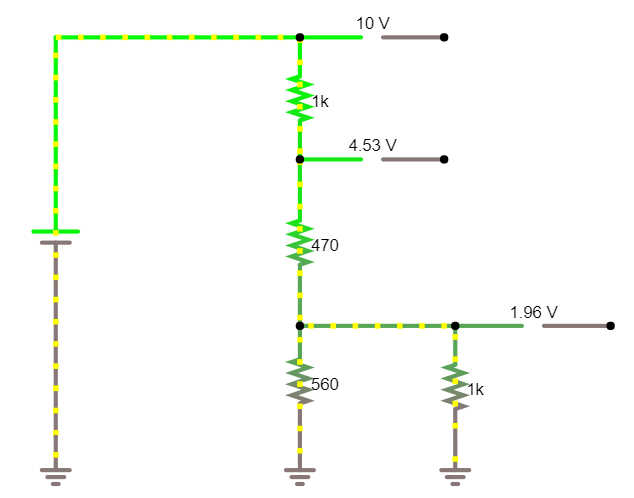
\includegraphics[width=\linewidth]{sims/Vnodes}
\caption{Voltages in nodes}
\end{subfigure}
\begin{subfigure}{0.48\textwidth}
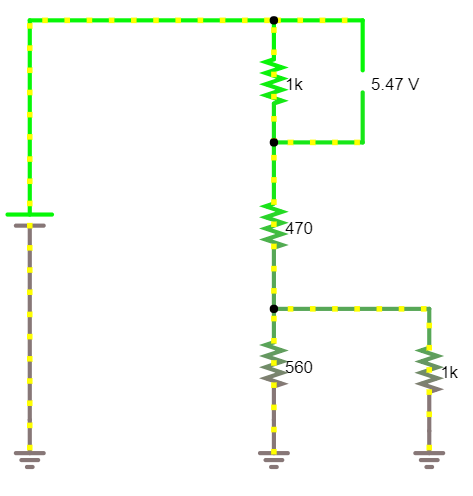
\includegraphics[width=\linewidth]{sims/VR1}
\caption{Voltage in $R_1$}
\end{subfigure}
    \caption{Simulations for voltage values (nodes and $R_1$)}
\end{figure}
\begin{figure}[H]
\begin{subfigure}{0.48\textwidth}
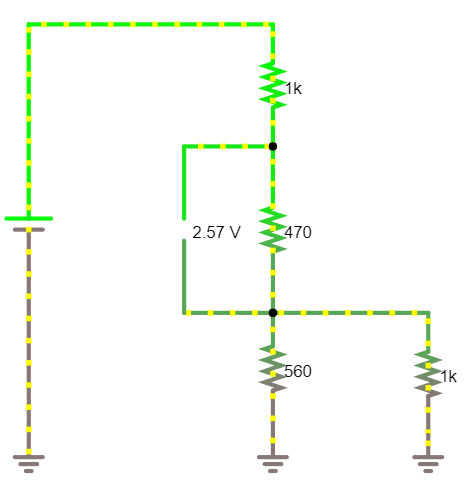
\includegraphics[width=\linewidth]{sims/VR2}
\caption{Voltage in $R_2$}
\end{subfigure}
\begin{subfigure}{0.48\textwidth}
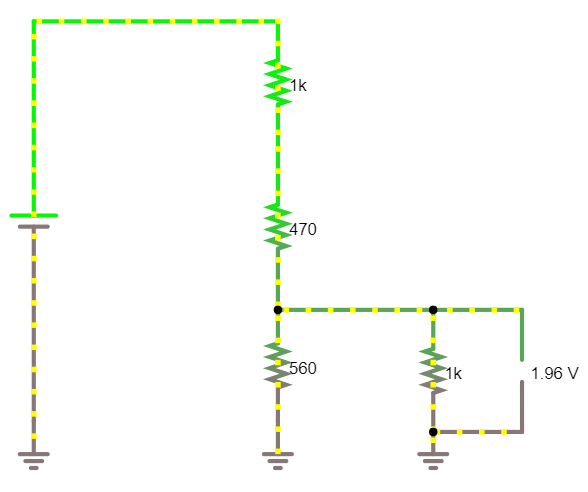
\includegraphics[width=\linewidth]{sims/VR3}
\caption{Voltage in $R_3$}
\end{subfigure}
    \caption{Simulations for voltage values ($R_2$ and $R_3$)}
\end{figure}
\begin{figure}[H]
\begin{subfigure}{0.48\textwidth}
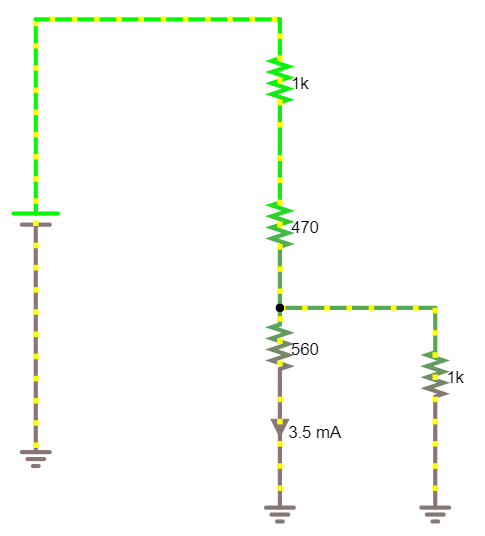
\includegraphics[width=\linewidth]{sims/IR3}
\caption{Current in $R_3$}
\end{subfigure}
\begin{subfigure}{0.48\textwidth}
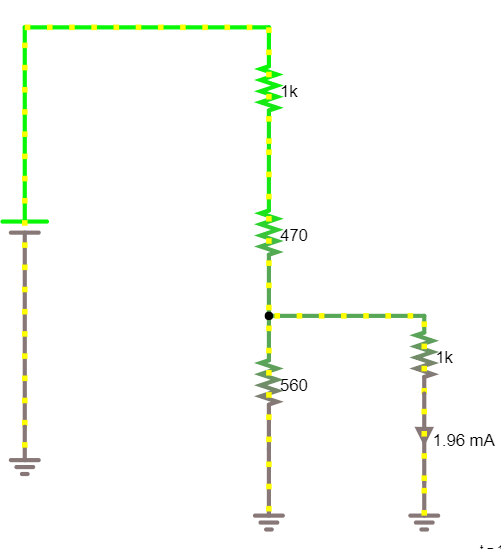
\includegraphics[width=\linewidth]{sims/IR4}
\caption{Current in $R_4$}
\end{subfigure}
    \caption{Simulations for current values}
\end{figure}
    \begin{figure}
    \centering
        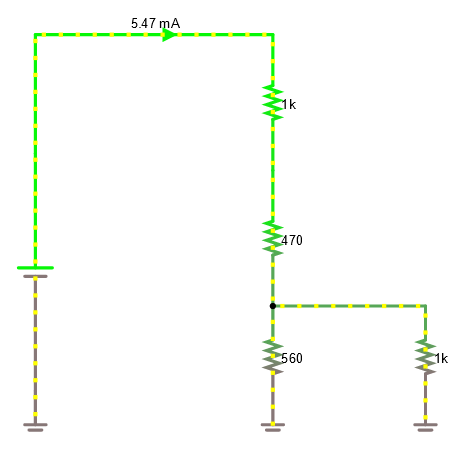
\includegraphics[width=0.48\textwidth]{sims/Itot}
        \caption{Simulation for total current}
    \end{figure}
\subsubsection{Measurements}
\begin{table}[H]
    \centering
    \begin{tabular}{|c|c|c|c|c|}
    \hline
    Measurements & Theoretical & Measured & Simulated & Error($\Delta V$)\\
    & Value & Value & Value & \\\hline
    $V_1$ & $\SI{10}{\volt}$ & $\SI{10}{\volt}$ & $\SI{10}{\volt}$ & $\SI{0.163}{\volt}$\\\hline
    $V_2$ & $\SI{4.533}{\volt}$ & $\SI{4.370}{\volt}$ & $\SI{4.530}{\volt}$ & $\SI{0.415}{\volt}$\\\hline
    $V_3$ & $\SI{1.963}{\volt}$ & $\SI{1.548}{\volt}$ & $\SI{1.960}{\volt}$ & $\SI{0.087}{\volt}$\\\hline
    $V_{R1}$ & $\SI{5.467}{\volt}$ & $\SI{5.538}{\volt}$ & $\SI{5.470}{\volt}$ & $\SI{0.071}{\volt}$\\\hline
    $V_{R2}$ & $\SI{2.570}{\volt}$ & $\SI{2.860}{\volt}$ & $\SI{2.570}{\volt}$ & $\SI{0.290}{\volt}$\\\hline
    $V_{R3,R4}$ & $\SI{1.963}{\volt}$ & $\SI{1.598}{\volt}$ & $\SI{1.960}{\volt}$ & $\SI{0.365}{\volt}$\\\hline
    $I_{R3}$ & $\SI{3.504}{\milli\ampere}$ & $\SI{3.590}{\milli\ampere}$ & $\SI{3.500}{\milli\ampere}$
    & $\SI{0.086}{\volt}$\\\hline
    $I_{R4}$ & $\SI{1.963}{\milli\ampere}$ & $\SI{1.490}{\milli\ampere}$ & $\SI{1.960}{\milli\ampere}$
    & $\SI{0.473}{\milli\ampere}$\\\hline
    $I_T$ & $\SI{5.467}{\milli\ampere}$ & $\SI{5.080}{\milli\ampere}$ & $\SI{5.470}{\milli\ampere}$ &
    $\SI{0.337}{\milli\ampere}$\\\hline
    \end{tabular}
    \label{tab:1}
    \caption{Measured, simulated and calculated voltage values and their error}
\end{table}
\section{Questions}
\textit{\textbf{Why does the deviation between the measured values and calculated values exist?}}

It’s meant to be a reference about “how much” is an error acceptable or not. It can help the user
to see if he or she is reaching the desired results with a pretty simple (but precise)
procedure.\\
\textit{\textbf{In electric circuits analysis, what is the voltage divider useful for?}}

Voltage dividers have tons of applications, they are among the most common of circuits electrical
engineers use. It makes circuit analysis way more simple in a lot of cases (but obviously not
every single time). It’s used to dive a big voltage into a “smaller” one between to resistors
through a simple equation.\\
\textit{\textbf{Can the voltage divider of an electric circuit be extended to a greater amount of
resistors?}}

Yes, as long as all of them are connected in a way  that the electric circuit can still be
analyzed with the voltage divider. This condition is for the circuit to be connected in
series.\\
\textit{\textbf{If the need to predetermine the voltage in every node existed, what should be done to
obtain said values?}}

For the value in the upper node we need to set the voltage source with the
same value, then, for the following nodes, depending on their value, we need to find the
right resistor or combination of them so the voltage $V$ is equal to $V_0-R\cdot I_T$, where
$V_0$ is the voltage of the previous node, $I_T$ is the total current flowing
through the circuit and $R$ is the total resistor between the nodes $V_0$ and $V$, and then
repeating the same procedure in the following nodes.
\section{Conclusions}
{\large\textbf{Sabrina:}}\\
Voltage Divider Is one of the easiest tools out there to analyze electric circuits. It is also one of the most used “resistors simplifier”. Thus, the engineer can add this method to the collection for solving real and theoretical problems.
\\[2ex]
{\large Salvador:}\\
The voltage divider is a very useful tool to find the theoretical measurements in the electrical circuit and the practical measurements in this practice
and in everyday life has many applications such as the potentiometer.
\\[2ex]
{\large Sebastián:}\\
We used the voltage divisor equation to calculate voltage values in our circuit, we did this because
it was composed by resistors wired in series, only one of the resistors were wired in parallel to
other resistor, this allowed us to get the values without going through the process that implies
mesh analysis or node analysis, therefore reducing the time consumed doing calculations. Finally, to
obtain other values such as voltages in nodes or current in resistors, we made substractions
depending on the node and used Ohm's law respectively.
\end{document}
